\chapter{Concluding remarks}\label{ch:conclusion}

\setlength{\epigraphwidth}{0.49\textwidth}%0.57
    \setlength{\epigraphrule}{0pt}%0.1
    \epigraphhead[5]{%
    \epigraph{\emph{Has been done. Can be done. Must be done\ldots}}%
    {Fandarel \mycite{McCaffrey}}
}

With the recent profusion of expression atlases
and the steadily growing number of independent studies
integrating data from these atlases as-is\footnote{%
More than 3,000 citations on 4 November 2019 for five human studies~\mycite{%
castleData,VTpaper,Uhlen2014,Uhlen2015,GTExTranscript}.},
it has become increasingly imperative to examine
the soundness of their extensive use.\mybr\

At the time I started my doctorate,
no assessment on the robustness of expression or
comparison between independent \Rnaseq\ datasets was published yet.
My primary aim was to provide an overview
by integrating and comparing independent transcriptomic data
of undiseased human tissues.
However, the release of two substantial proteomic datasets in the meantime
broadened my study's scope
to include the integration of transcriptomic with proteomic data as well.\mybr\

%\vspace{-2mm}
\section*{Summary}
%\vspace{-5mm}
In \Cref{ch:background},
I reviewed the biological, chemical and bioinformatic aspects and challenges
involved in expression studies based on the high-throughput technologies
of \Rnaseq\ for \mRNAs\ and \ms\ for proteins.\mybr\

Then in \Cref{ch:datasets},
I presented the five transcriptomic and three proteomics studies
that I have considered for this thesis.
I also described the pipelines with which I have processed them.
Since for each dataset the number and size of files are extremely large,
automation is paramount to ensure consistency and minimise errors.\mybr\

I detailed in \Cref{ch:expression} various data quality controls
and statistical approaches.
I also discussed possible biases and
how the contextual scope of the tissues and genes considered for analyses
can influence results.
To minimise errors due to context issues,
I limited most of my further investigations to
a common subset of tissues and expressed genes.
Normalisation methods are still inadequate
to treat mitochondria genes accurately.
Therefore, I chose to remove them from most analyses,
which led to better results
as it allowed me to integrate samples
that the original authors had to discard
because of their lack of congruency with the other samples of the same tissue.\mybr\

In \Cref{ch:Transcriptomics},
I integrated the five independent transcriptomic datasets and
showed that the biological signal dominates the technical noise.
All datasets have a higher interstudy correlation for the same tissues
than any intrastudy correlation for different tissues.
This trend is stronger for more recent studies.
I tested various criteria as possible driving forces
of the high interstudy tissue correlations.
I found that the most variable genes and tissue-specific (\gls{TS}) genes
are individually contributing more to the high correlations
than the highest expressed ones.
Besides, I also noted that
the inclusion of external resources,
especially when outdated like \gls{TIGER}~\mycite{tiger},
requires caution.
Many listed genes are either wrongly attributed to a tissue
or lack to display any specificity and
many \gls{TS} genes highlighted by \Rnaseq\ are missing.
Overall, the integration has revealed that
genes present identical general profiles across the studies,
even though direct comparisons of independent data may be still impossible.
By repeatedly showing that
genes show a similar expression profile for a tissue across studies,
my analyses prompted the creation of the heatmap visualising expression data
and its associated widget for baseline expression data in
\hFoCi{EBI Expression Atlas}{https://www.ebi.ac.uk/gxa/home}{EBIgxa}.
Finally, I provided a core set of genes that are expressed
ubiquitously or as \gls{TS} consistently across all studies.\mybr\

The comparison of three available proteomic datasets
in \Cref{ch:proteomics} highlights
the fragmentation and the disparity of the high-throughput \ms{}-based proteomics.
\ms\ detection variability induces considerable technological noise,
which explains
the intrastudy correlations I observed between different tissues are
higher than the interstudy correlation for the same tissues.
I provided curated sets of the \gls{TS} and ubiquitous detected proteins.
Finally, I have invented the \PPKM\ quantification method,
which quantifies more proteins by also accounting for degenerated peptides.\mybr\

\Cref{ch:Integration} reported
the integration of the independent proteomic and transcriptomic data.
Regardless of the quantification method,
I found for these independent studies
similar Spearman correlation levels
to those typically observed in the literature
for same-sourced proteome and transcriptome source.
While proteomic standard state-of-art processing leads
to very low Pearson correlation: $0.04 ≤ r ≤ 0.28$,
our \PPKM\ quantification broadly improves this range ($0.38 ≤ r ≤ 0.61$).
Two tissues, \Testis\ and \Liver,
have exhibited distinct characteristics across the various analyses
that are supported by the literature.
\Testis\ has the most diverse and specific expression
at both transcriptomic and proteomic levels.
On the other hand, \Liver\ has the most robust expression across studies
and the highest correlation between its \mRNAs\ and proteins expression levels.
Overall, the tissues show mixed correlation levels,
and it is impossible to predict protein expression accurately
from \mRNA\ levels alone.
However, there are shared coherent gene signatures
between the proteome and transcriptome.
Furthermore, even indirect analyses can capture part of the biological signal.
Proteins' and \mRNAs{}' tissue specificity are contributing
more to the tissue correlation than their expression levels once again.
In addition to the significant overlaps of \gls{TS} proteins
with the most \gls{TS} \mRNAs,
most genes with a \gls{TS} protein have
a high correlation between their \mRNA\ and protein expression across tissues.
\gls{go} analyses show distinct profiles for three gene lists of interest.
First, the genes with a \gls{TS} protein
are enriched for specific signalling,
including signal detection, response pathway and regulation.
Second, the genes with the highest correlations
between their \mRNA\ and protein expression
are enriched for catabolic processes.
Thirdly, the genes with the highest anticorrelation
between their \mRNA\ and protein expression
have shown enrichment for ribosome complexes and \glspl{ncRNA} regulation.
I provide the complete set of \mRNA/protein pairs with their correlation
across the common set of tissues.
I also supply the list of overlapping \gls{TS} proteins and \mRNAs{}.\mybr\

\section*{Practical challenges}
Throughout this thesis' analyses,
I had to overcome many practical challenges.
While most of the difficulties encountered ordinarily pertain to Big data projects,
one unexpected issue was
the current global complexity state of the proteomic world.\mybr\

%\vspace{-3mm}
\subsection*{Proteomics: a hard field to grasp by newcomers}
\vspace{-6mm}
While constituting a technical obstacle,
the characterisation of proteins (or assimilated complexes)
is a strong interest for many fields
(\eg\ molecular biology, medicine, drug design, green chemistry).
As shown in \Cref{sec:exploreProtMS},
the physicochemical properties of the proteins make them
intrinsically complex to study,
which can partly explain the complexity of the theoretical approaches.
Understanding high-throughput proteomics requires many prerequisites.
However, there is a lack of a clearly identified entry-level document
reviewing the field from the bench to normalised protein levels.
The available teaching materials are mostly
practical or experimental oriented~\mycite{Zhang2013,Zhang2014,LCMSconsider} or
on particular steps, \eg\ protein inference~\mycite{He2016-yi}.
The scattered information hampers the ability of newcomers
to achieve a global vision of high-throughput proteomics.\mybr\

\subsection*{Big data Challenges}
\vspace{-6mm}
Big data is often characterised through, what was first defined by
\href{https://www.ibmbigdatahub.com/infographic/four-vs-big-data}{IBM}\footnote{%
\Href{https://www.ibmbigdatahub.com/infographic/four-vs-big-data}},
the \emph{4 V's}: volume, variety, veracity and velocity.
Each of them can entail issues at different project levels.\mybr\

\subsubsection*{Volume}
\vspace{-3mm}
The volume of files (see \Cref{tab:Lib5DF})
to handle and process just for the transcriptomics
is overwhelming and requires properly dimensioned infrastructure
like in the \gls{EBI}, which can provide high-throughput computing.
It is in practice impossible to reproduce the complete work underlying
this thesis in a personal computer within a reasonable time.
Although (commercial) solutions are increasingly in use for academic projects,
dedicated storage and high computing facilities ease the analyses considerably
and allow more in-depth testing.
Even if best practices are continuously refined for transcriptomics,
there are still many factors that can be improved and tuned.
Besides the raw data,
storage capacity is also required for the intermediate and final files.
Organising such a large amount of data was time-consuming and
challenging at times.\mybr\

\subsubsection*{Variety}
\vspace{-3mm}
The variety of the type of input data files is kept to a minimum
as the data was retrieved from public or academic repositories
that follow community guidelines\footnote{%
\href{https://www.ebi.ac.uk/ena}{ENA} for the sequencing data and
\href{http://www.proteomexchange.org}{ProteomeXchange} for \ms/\ms\ proteomics.
}.
Issues still ensued from the matching of samples or tissues across the studies.
For many tissues, I chose to mix several \enquote{body parts}
from the same tissue or organe
(\eg\ \enquote{Left Ventricle} and \enquote{Atrial Appendage} for \Heart) in \gtex\
to match them to the other studies' tissues.
Perhaps, in some case, one \enquote{body part} is perfectly matched
to the samples from another study
where the authors have only reported the tissue instead.
Hence, for these cases,
keeping only one of the \enquote{body parts}
would have been a better choice.\mybr\

Another source of variety that I have limited in the above work
is the diverse annotation versions.
Even when mapped to the same genome and annotation versions,
discrepancies persist between how transcriptomics and proteomics
are defined and assigned to the genes.
A possible improvement of the present work will be to use
the chromosome coordinates to which \mRNAs\ and proteins map
instead of using their gene identifiers.\mybr\

\subsubsection*{Veracity}
\vspace{-3mm}
Additionally, with all possible tunable parameters for the raw data processing,
the data to be integrated can vary widely.
Even with a limited number of combinations,
my study shows that the results' trend remains the same
regardless of the chosen settings.
Moreover, as the number of datasets I included in my analyses grows,
the results became increasingly more stable.
Many of them have also been confirmed by the literature,
adding credibility and confidence to the findings,
especially considering the recent discussions on reproducibility crisis~\mycite{%
Morrison2014-hy,Glenn_Begley2015-fz,Goodman2016-ri,Fatovich2017-lo,
Coiera2018-vf,Lindner2018-qy}.
However, results for individual genes can vary from one set of settings to another one,
and need to be considered with more caution.\mybr\

\subsubsection*{Velocity}
\vspace{-3mm}
Finally, the velocity of new data availability
and the required preparation time
made the prospect of including all the latest studies in my analyses impractical.
Unfortunately, although new \gtex\ samples or other tissue studies
(\eg\ Oncobox Atlas of Normal Tissue Expression (ANTE)~\mycite{Suntsova2019-it})
kept being released,
I had to stop including them in my study.
Likewise, I ceased updating the genome and annotation
and settled for \hg{38.p1} and \ens{76}.\mybr\

\subsubsection*{My resolving approach}
\vspace{-3mm}
To minimise errors,
assure consistency and ease future reiterations or extension of these analyses,
I provide script files that can reproduce the whole study and its results.
I have also automated and structured the analyses through modular functions
as much as possible.
I have avoided any manual change and
have documented all the name change and sample pairings in the scripts.
I provide the necessary code to replicate all of the above (and complementary) results
as \href{https://github.com/barzine/BaselineAtlas/tree/thesis.}{supplementary
material}\footnote{\Href{https://github.com/barzine/BaselineAtlas/tree/thesis}}.\mybr\

I chose to develop the analyses with open-source software
around the programming language \WebFoCi{\textsf{R}}{https://cran.r-project.org}{coreR}.
See \Cref{sec:Rpackages} for the complete list of \textsf{R} packages
involved in this work.
This language provides statistical and visualisation functions
and is easily expanded through packages developed by the community.
Packages can be highly interdependent and may evolve rapidly.
To draw from an extra package (or fix an identified bug),
a comprehensive and time-consuming update of the working environment
will often ensue.
In turn, I had also to update my analyses' code on many occasions.
Furthermore, new software installations or updates are more complicated
for distributed computing facilities than on a personal computer.
Today, new solutions are developed to facilitate these tasks
(\eg\ \softCi{Packrat}{Rpackrat} that create isolated environment).\mybr\

Note that \nuno, who provided me with the quantification of the \gtex\ data,
and \james, who provided me with the proteomics ones,
have also both developed their processing pipelines with open-source software.
Hence, the entirety of the thesis (subject to access to \gtex\ data)
can be repeated easily.\mybr\

\section*{Future works}
Many improvements are conceivable:\mybr\
%\vspace{-3mm}
\begin{itemize}[topsep=0pt,nosep]
        \item The inclusion of new samples and dataset of transcriptomics
            (preferably with biological replicates),
            \eg\ extend to the last version of \gtex\ and
            the ANTE dataset~\mycite{Suntsova2019-it}.
        \item Add the matching proteomics of \citet{Wang2019-ut}
            to the transcriptomic \uhlen\ data~\mycite{Uhlen2015}
            and then compare the results to the unmatched samples.
        \item Work on new models of annotation or
            build a consensus between the current transcriptomic and proteomic
            annotations.
            Today, it is difficult to determine for some genes
            if the observed anticorrelation or lack of correlation
            between the \mRNA\ and protein expression levels is due to the biology,
            batch effects or divergences between transcriptomic and
            proteomic annotations.
        \item Changing the quantification (parameters or methods)
            may also give better results.
\end{itemize}
%The potential for improvement due to quantification is appealing.\mybr\

\subsection*{New quantification proposal for baseline studies}
\vspace{-6mm}
Most normalised quantification methods are designed
for differential expression studies,
particularly in transcriptomics~\mycite{Dillies2013}.
Most of these methods are built with the premise
that only a limited number of genes present a differential expression across conditions
while most gene expressions remain unaffected by the context~\mycite{licomparing:2015}.
As a result, most normalisations are ill-suited
for comparing independent samples across multiple studies.
Two normalisation methods do not imply any preconception on the study design:
\gls{FPKM}~\mycite{Mortazavi2008,cufflinks} (see \Cref{subsub:norm}),
which I use in this thesis,
and TPM (Transcript per Million)\footnote{%
\FPKM\ is easily converted to TPM by scaling with a constant
to correct the sum of all values in a library to 1 million.
}~\mycite{Wagner2012-du}.
Both normalisation methods account for the global library size of each sample.
While the motivation is sound,
the quantification is thus contextual
to %which
how many
and how much \glspl{RNA} are detected.\mybr\

Previous efforts to solve this problem have focused
on differential expression studies.
Synthetic spike-in molecules~\mycite{Jiang2011-ux}
ensure more reliable quality controls.
However, while theoretically plausible,
accurate absolute quantification for the whole dynamic expression range
has yet to be reached~\mycite{Jiang2011-ux,seqcmaqc,Hardwick2017-ib}.
Furthermore, spike-ins fail to permit the absolute quantification
of the other molecules in the sample.
Incidentally, \citet{Rudnick2014-ar} find that spike-in proteins and peptides
lack effectiveness for proteomic studies.
For proteomics, \citet{Wisniewski2014-kh} propose
to use the histone to create a \enquote{\emph{proteomic ruler}}.
They can assess through this proteomic ruler the amount of \gls{DNA}
in the sample, and thus, give an estimate on the cell number,
which provides some context to interpret the quantification of the proteins.
Histone genes are, however, ill-suited
for bulk \Rnaseq\ studies~\mycite{Zhao2018-rw}.\mybr\

I firmly believe that using internal standards chosen
within the naturally expressed population of the studied macromolecules
is more appropriate than any external additive.
I expect that giving each gene (RNA or protein) expression
as a ratio of the expression of a reference gene will be more robust.
It will free the expression
from the influence of the presence of quantification of any other gene
while it will still account for the difference of sequencing depth between samples.
Then, the next question is:
\enquote{Which gene (or set of genes) will possibly enable the best normalisation?}\mybr\

Through this thesis' various analyses,
I have highlighted genes that have a robust and ubiquitous expression
across all the studied tissues
both at transcriptomic and proteomic levels.
Moreover, many genes present high correlation coefficients
between the expression of their \mRNA\ and protein.
These genes are the best potential candidates as reference.
With \nuno, we have performed preliminary analyses
in this direction across other studies
to reduce the list of these candidates.\mybr\

However,
considering the best practices in analytical chemistry~\mycite{analyticalChem},
a set of standards that can cover the complete dynamic expression ranges
of the considered molecules
and adjust for the saturation effects,
may resolve the abundances better,
and thus, be better suited than a single reference.
On the other hand, studies focusing on a single tissue
may better benefit from a reference built on \gls{TS} genes.\mybr\

The recent development of single-cell transcriptomics
(scRNA-Seq)~\mycite{Chen2019-um},
and the probable feasibility of single cells proteomics~\mycite{Marx2019-cf},
may ease refining which genes are the most suitable as universal references,
or for specific conditions.\mybr\


\subsection*{Ongoing implementation of an application}
\vspace{-6mm}
Integrating proteomics and transcriptomics remains laborious,
and results can be mixed.
Nonetheless,
even simple comparisons % of independent data
can help to improve our general knowledge
and current biological models.
For instance, in one of our papers % \citetitle{Wright-2016}
\mycite{Wright-2016},
we have confirmed the existence of putative proteins
by observing coverage of the genome both by transcriptomics and proteomics.\mybr\

%\vspace{-1mm}
To help further possible projects,
I am currently compiling the different analyses
into a set of interactive applications
that can replicate all the results and figures presented in this thesis
without requiring any programming skill as a prerequisite.
\Cref{fig:demoApp} covers \Cref{ch:expression}.\mybr\

%\vspace{-1.5mm}
\begin{figure}[!ht]
    \frame{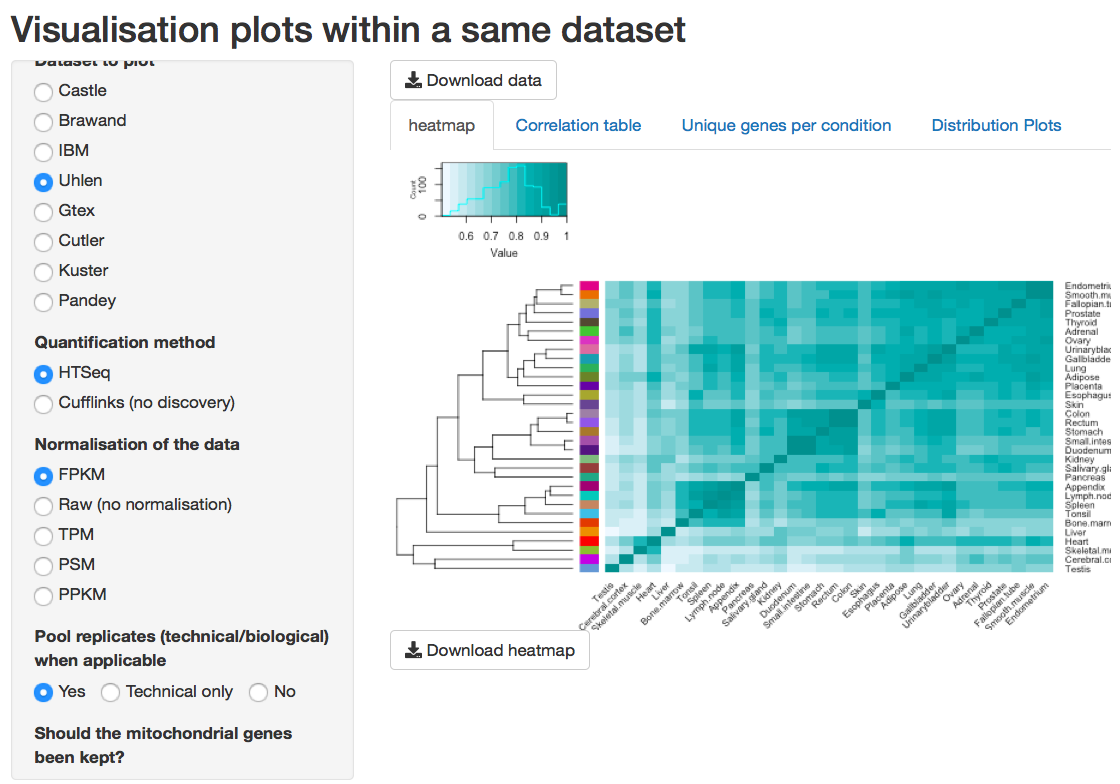
\includegraphics[scale=0.31]{conclusion/demoApp.png}}\centering
    \vspace{-2mm}
    \caption[Application preview]{\label{fig:demoApp}\textbf{Preview of the
    application} developed with \textsf{R}
    and served through a shiny server~\mycite{shinyR}.}
\end{figure}
%\vspace{-3mm}
Once completed, one will be able to analyse and compare their own data
to the different datasets I have presented in this thesis.
Furthermore, as I share all my code (including for the application)
under a creative commons license,
\WebFo{Attribution 4.0 International  (CC BY 4.0) 
\includegraphics[width=1em]{cc.pdf}%

\includegraphics[width=1em]{by.pdf}}{https://creativecommons.org/licenses/by/4.0}.
Anyone can thus use, adapt or build upon this work as they wish.\mybr\


%Achievements
% Showed that mitochondrial \mRNAs\ and proteins should be excluded from the bulk
% (even though separate analysis can be considered)
%
% Transcriptomics present similar profiles: tissue across datasets,
% and \mRNAs\ profiles through the tissues across datasets.
% This finding has prompted the EBI heatmap visualisation
%
% New proteomics quantification methods inspired on transcriptomic ones
% can increase the number of quantified proteins
% while seemingly unkooky
%
% First time so many different data have been mapped to the same genome version
% and annotation with identical pipelines.
% Quite in-depth comparison between Uhlen and \gtex.
% Reprocessing of all the untarget non-diseased human proteome
%
% Consolidated gene lists for consistent transcriptomic expression
%                                           (modified Uhlen categories)
%                 and for matched (but independently sourced) \mRNA/protein pairs
%                     for TS, highly correlated and very anticorrelated
%
% Organs show constant catabolic profile (set of genes) that have
% mRNAs/proteins expression consistent through aggregation of individual and
% across different datasets.
% Particularly, housekeeping and TS genes
%
% Testis most diverse and unique expression
% Liver most robust expression
%


